\setcounter{page}{2}
Целью лабораторной работы №1 является освоение возможностей программы Microsoft 
Project для планирования проекта по разработке программного обеспечения. 

\section{Задание для тренировки}

При создании плана проекта использовались параметры, заданные в Microsoft Project по умолчанию.
Настройки приведены на рисунке~\ref{fig:test_params}.

\begin{figure}[H]
	\centering
	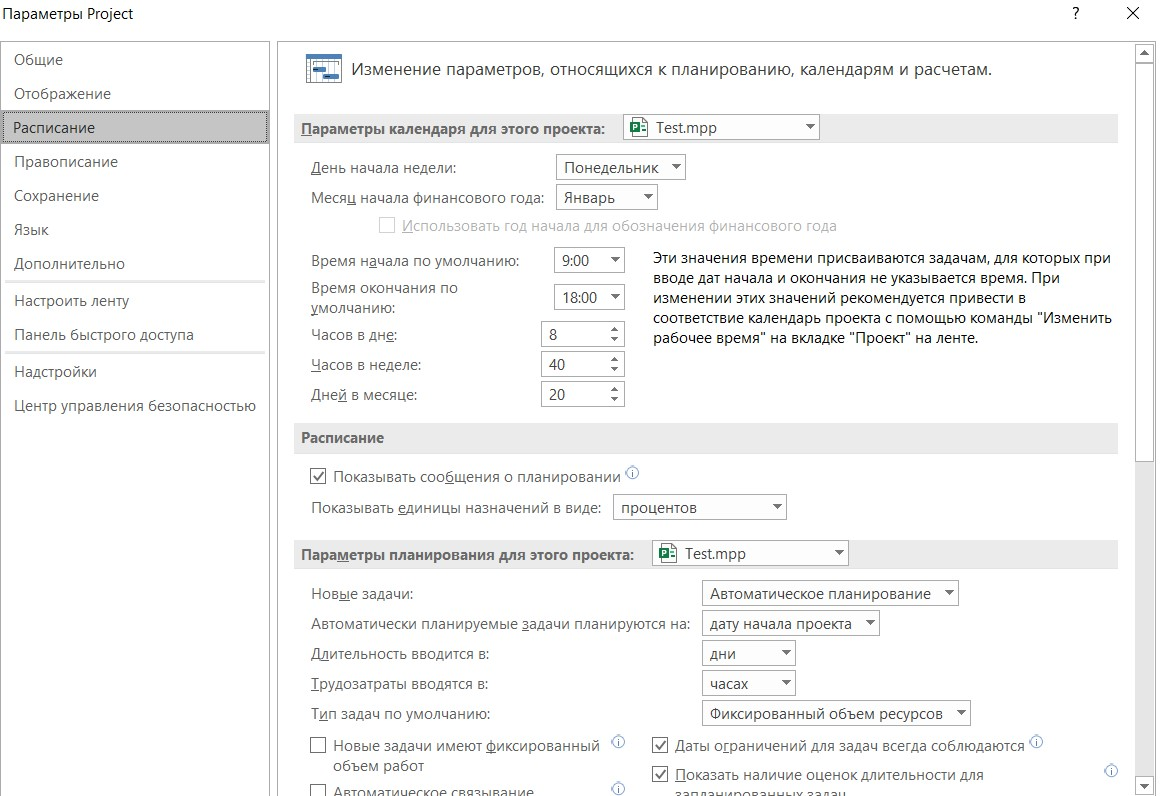
\includegraphics[width=0.9\textwidth]{img/test/params.jpg}
	\caption{Настройки проекта по умолчанию}
	\label{fig:test_params}
\end{figure}

По умолчанию рабочий день длится 8 часов с 9:00 до 18:00, в неделе 40 часов, что соответствует Трудовому кодексу.
Тип задач по умолчанию~---~с фиксированным объемом ресурсов, потому что чаще всего задано ограничение по ресурсам, а не по трудозатратам или длительности.

Датой начала проекта является первый рабочий день марта текущего года.
Настройка даты начала проекта представлена на рисунке~\ref{fig:proj_start}.

\begin{figure}[H]
	\centering
	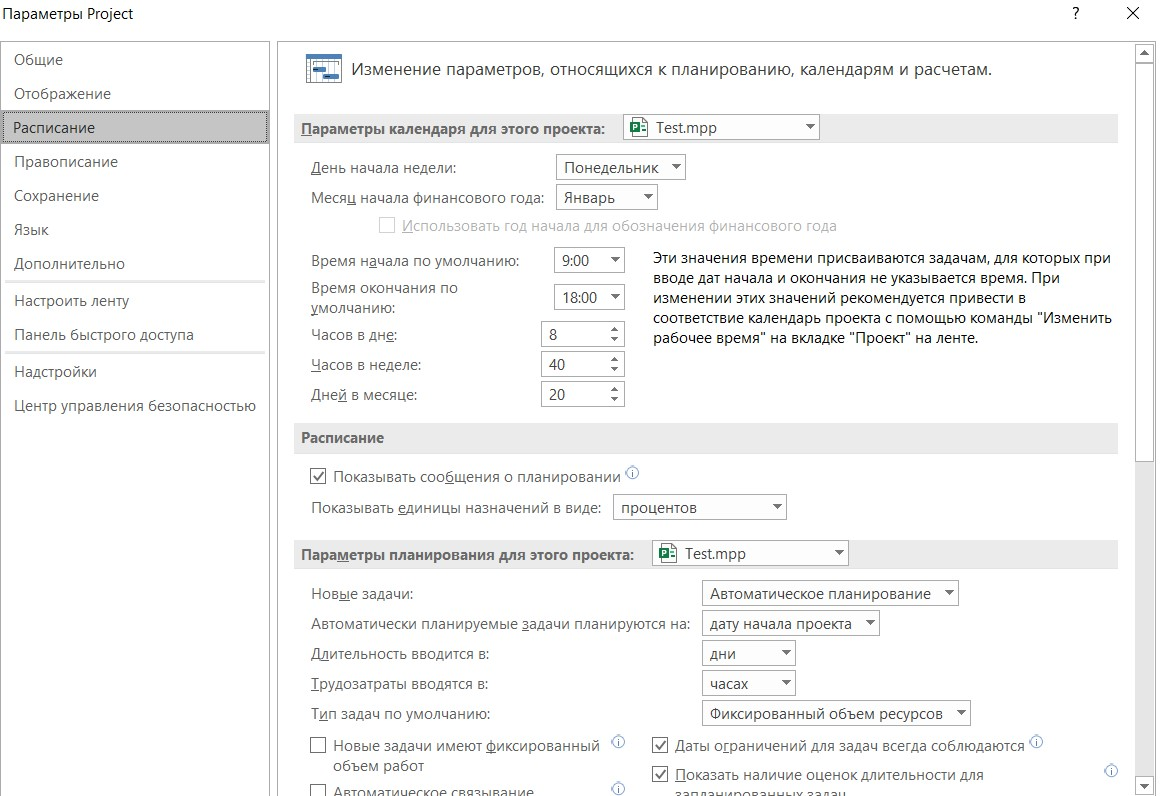
\includegraphics[width=0.9\textwidth]{img/test/params.jpg}
	\caption{Настройка даты начала проекта}
	\label{fig:proj_start}
\end{figure}

Временные характеристики проекта приведены в таблице~\ref{tbl:compare}.

\begin{table}[ht]
	\small
	\begin{center}
		\begin{threeparttable}
			\caption{Временные характеристики проекта}
			\label{tbl:compare}
			\begin{tabular}{|c|c|}
				\hline
				\textbf{Название работы}                                                & \textbf{\begin{tabular}[c]{@{}c@{}}Длительность (дни)\end{tabular}} \\ \hline
				\begin{tabular}[c]{@{}c@{}}Работа A\end{tabular}  & 12 \\ \hline
				\begin{tabular}[c]{@{}c@{}}Работа B\end{tabular}  & 6 \\ \hline
				\begin{tabular}[c]{@{}c@{}}Работа C\end{tabular}  & 10 \\ \hline
				\begin{tabular}[c]{@{}c@{}}Работа D\end{tabular}  & 7 \\ \hline
				\begin{tabular}[c]{@{}c@{}}Работа E\end{tabular}  & 9 \\ \hline
				\begin{tabular}[c]{@{}c@{}}Работа F\end{tabular}  & 8 \\ \hline
				\begin{tabular}[c]{@{}c@{}}Работа G\end{tabular}  & 10 \\ \hline
				\begin{tabular}[c]{@{}c@{}}Работа H\end{tabular}  & 10 \\ \hline
				\begin{tabular}[c]{@{}c@{}}Работа I\end{tabular}  & 6 \\ \hline
				\begin{tabular}[c]{@{}c@{}}Работа J\end{tabular}  & 5 \\ \hline
			\end{tabular}
		\end{threeparttable}
	\end{center}
\end{table}

На рисунке~\ref{fig:test} приведена построенная диаграмма Ганта.

\begin{figure}[H]
	\centering
	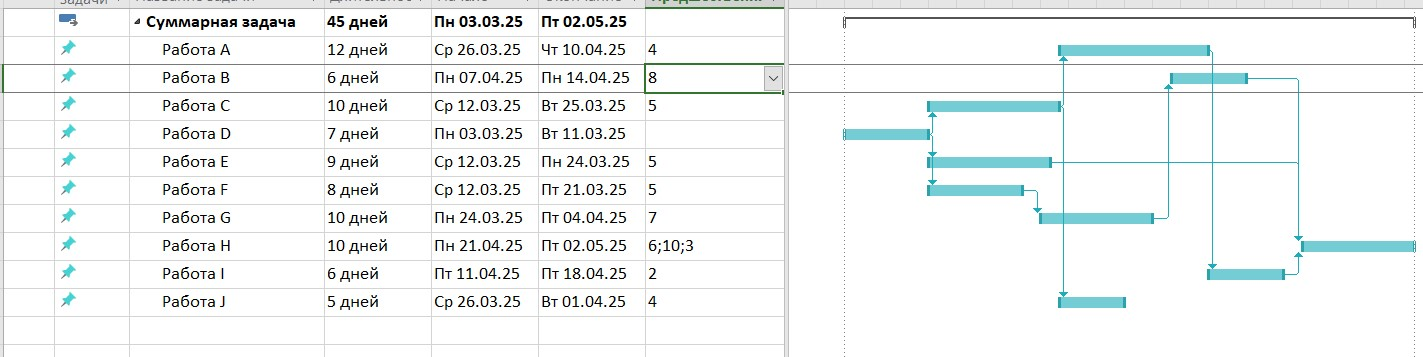
\includegraphics[width=0.9\textwidth]{img/test/test.jpg}
	\caption{Демонстрация выполнения задания для тренировки}
	\label{fig:test}
\end{figure}

Таким образом, определено, что длительность проекта для тренировки составляет 45 дней, дата его завершения~---~02.05.2025.

\section{Задание №1}

Проект представляет собой создание карты города.
В проекте участвуют 16 разработчиков, бюджет проекта~---~50000 рублей, длительность проекта~---~6 месяцев.
Дата начала проекта~---~первый рабочий день марта текущего года.

Перед добавлением задач необходимо настроить параметры проекта, находящиеся во вкладке $\text{Файл} \rightarrow \text{Параметры} \rightarrow \text{Расписание}$.
Настройка параметров представлена на рисунке~\ref{fig:parameters}.

\begin{figure}[H]
	\centering
	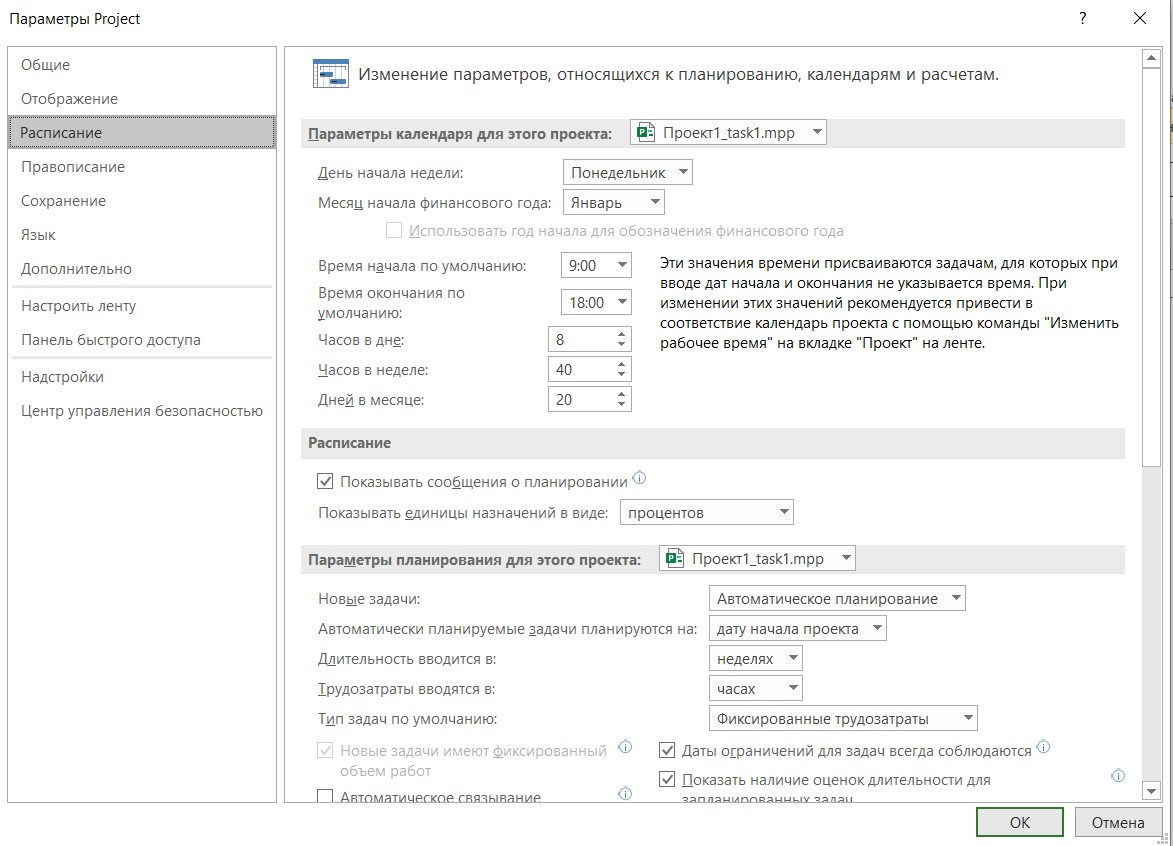
\includegraphics[width=0.9\textwidth]{img/task1/parameters.jpg}
	\caption{Настройка параметров проекта}
	\label{fig:parameters}
\end{figure}

Также необходимо внести в календарь праздничные дни и предшествующие им дни с укороченным рабочим графиком.
Для планируемого проекта такими днями являются майские праздники, день России в июне и день народного единства в ноябре.
Настройка календаря проекта приведена на рисунке~\ref{fig:calendar}.

\begin{figure}[H]
	\centering
	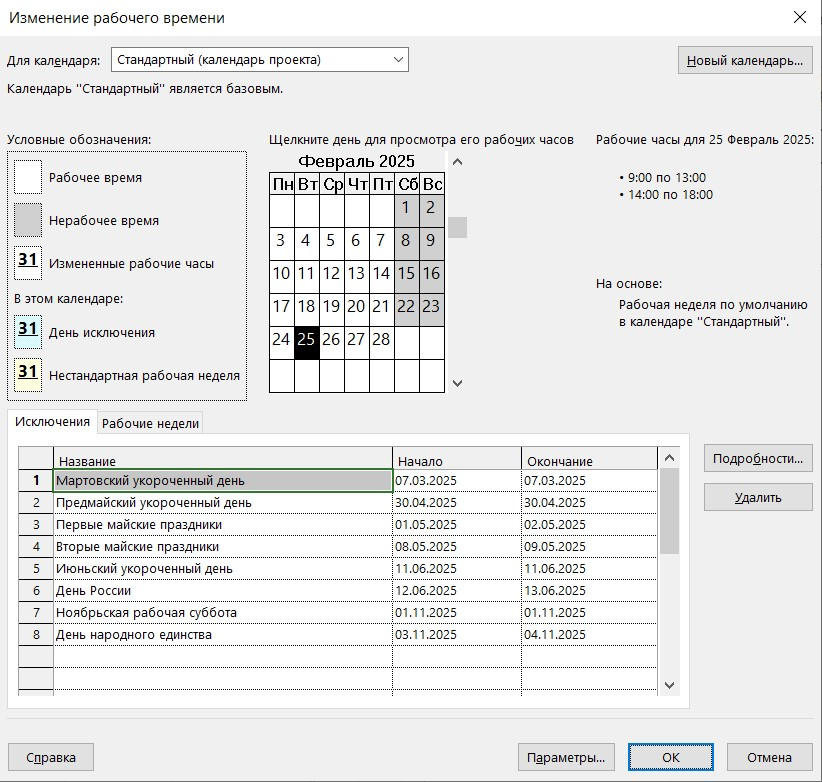
\includegraphics[width=0.9\textwidth]{img/task1/calendar.jpg}
	\caption{Настройка календаря проекта}
	\label{fig:calendar}
\end{figure}

Информацию о проекте можно посмотреть в Заметках, приведенных на рисунке~\ref{fig:notes}.

\begin{figure}[H]
	\centering
	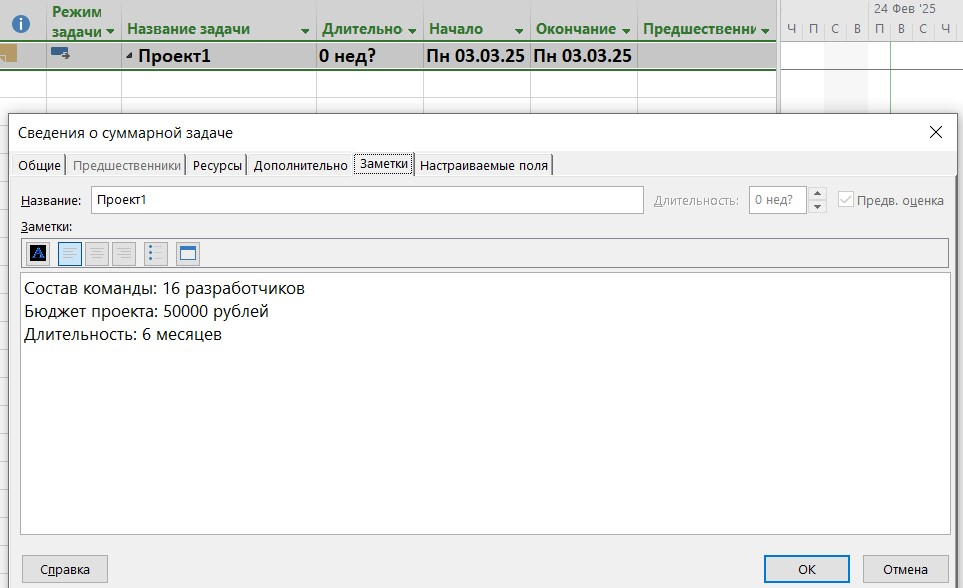
\includegraphics[width=0.9\textwidth]{img/task1/notes.jpg}
	\caption{Заметки проекта}
	\label{fig:notes}
\end{figure}

\section{Задание №2}

После настройки параметров проекта необходимо добавить задачи.
Так как в настройках указано, что автоматически планируемые задачи планируются на дату начала проекта, все задачи начинаются с третьего марта, что видно по диаграмме Ганта и столбцу <<Начало>> на рисунке~\ref{fig:task2}.

\begin{figure}[H]
	\centering
	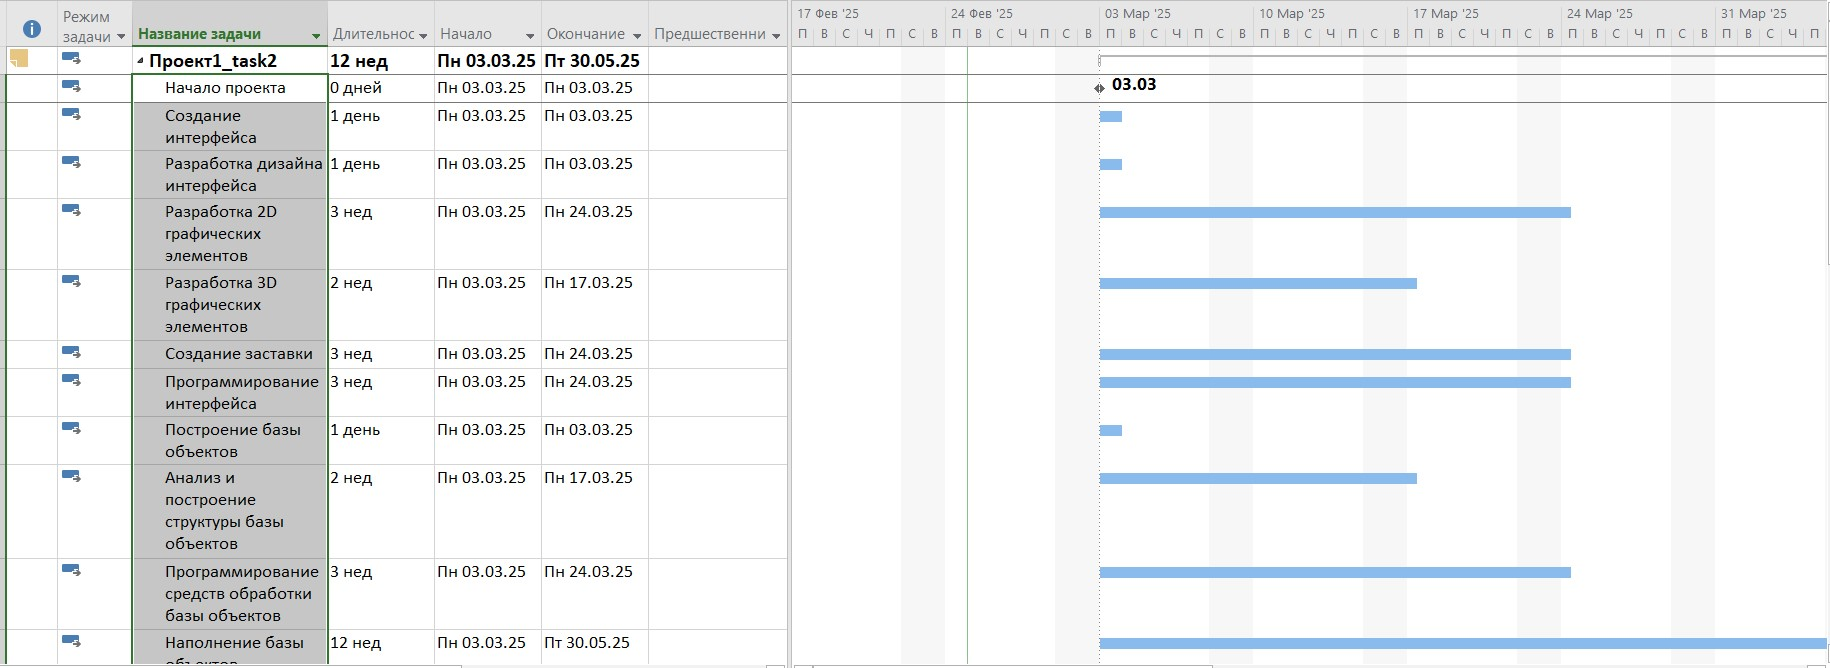
\includegraphics[width=0.9\textwidth]{img/task2/tasks.jpg}
	\caption{Диаграмма Ганта}
	\label{fig:task2}
\end{figure}

\section{Задание №3}

При проведении структурирования списка задач были выделены фазы проекта.
Результат структурирования списка задач приведен на рисунке~\ref{fig:task3}.

\begin{figure}[H]
	\centering
	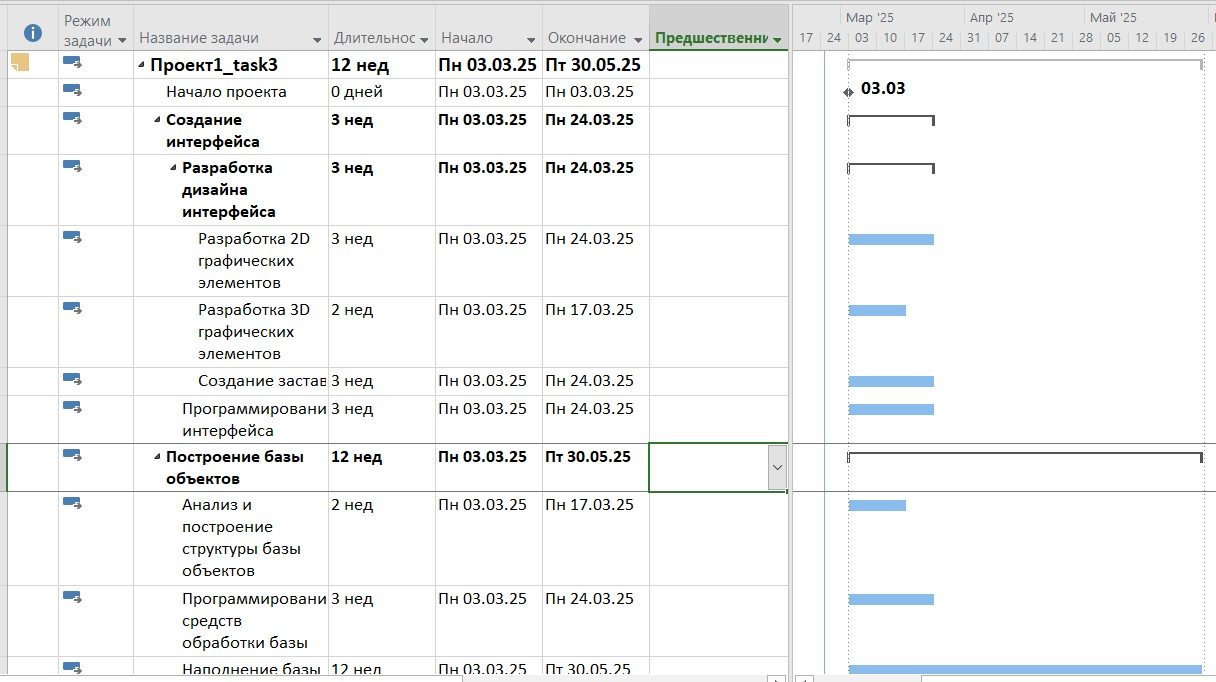
\includegraphics[width=0.9\textwidth]{img/task3/task3.jpg}
	\caption{Диаграмма Ганта после структурирования списка задач}
	\label{fig:task3}
\end{figure}

\section{Задание №4}

После структурирования списка задач необходимо указать связи между ними. 
Предшествующие задачи можно указать в столбце <<Предшественники>>.
По умолчанию устанавливается тип связи Окончание~---~Начало, при котором последующая задача начинается после окончания предыдущей.
В случае необходимости выбора другого типа связи необходимо дважды кликнуть по связи между задачами на диаграмме Ганта.
В появившемся модальном окне можно выбрать тип связи, а также указать время опережения/запаздывания.

Результат настройки связей между задачами приведен на рисунках~\ref{fig:task41} и~\ref{fig:task42}.

\begin{figure}[H]
	\centering
	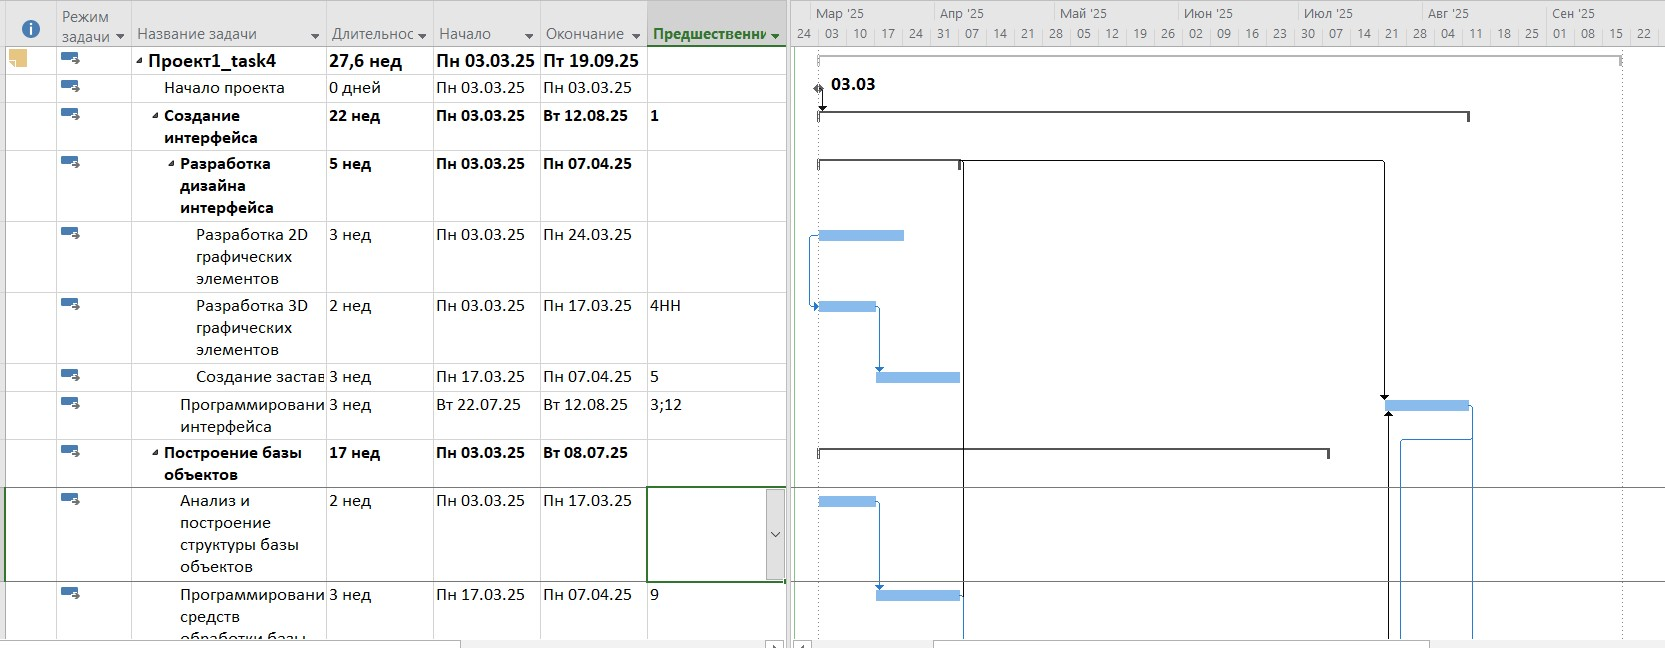
\includegraphics[width=0.9\textwidth]{img/task4/task4.jpg}
	\caption{Диаграмма Ганта с датой начала проекта}
	\label{fig:task41}
\end{figure}

\begin{figure}[H]
	\centering
	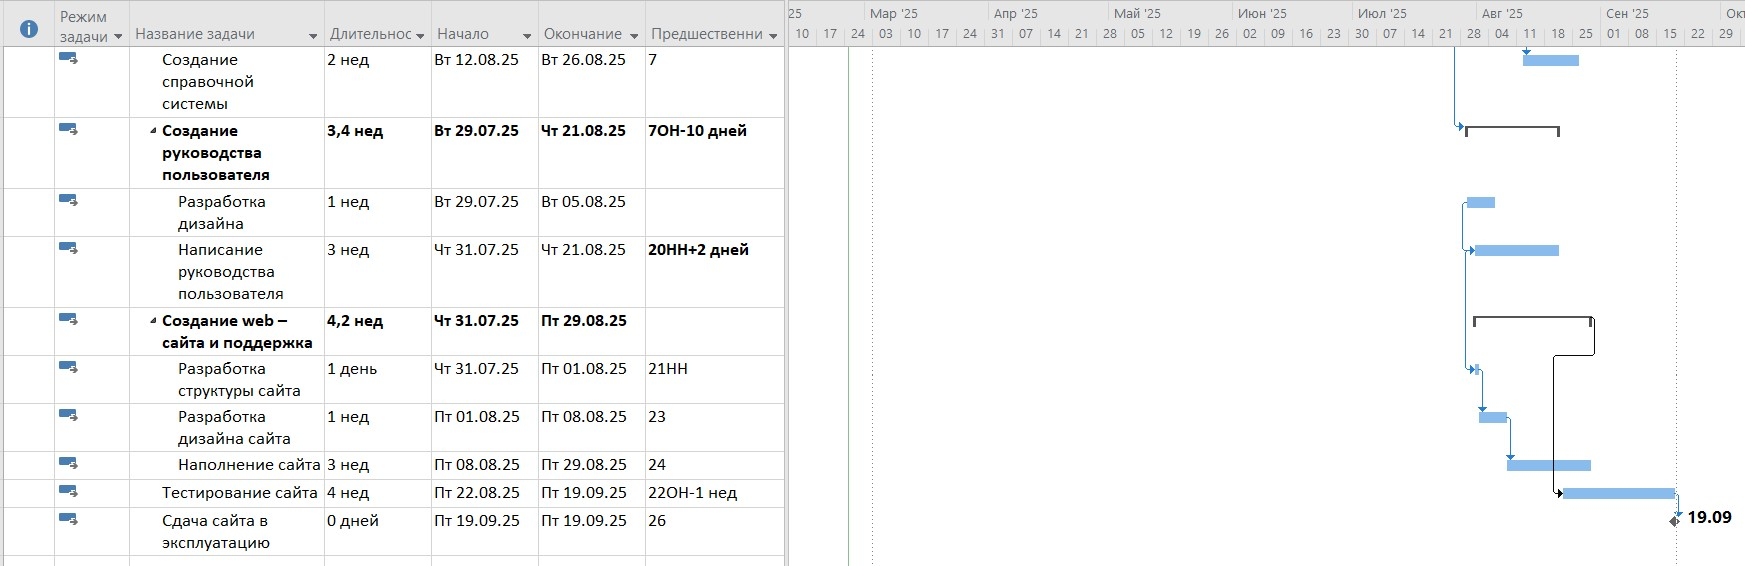
\includegraphics[width=0.9\textwidth]{img/task4/task4_1.jpg}
	\caption{Диаграмма Ганта с датой завершения проекта}
	\label{fig:task42}
\end{figure}

В результате планирования проекта было определена дата завершения проекта: 19 сентября 2025 года.
Таким образом, проект не уложился в срок 6 месяцев.